\chapter{Grundlæggende}

\section{Hvad er en graf?}%
\label{sec:label}

Königsberg-problemet er ofte sagt til at være problemet der ``startede'' graf-teori. Beboerne af Königsberg i Preussen (i dag er dette \href{https://en.wikipedia.org/wiki/Kaliningrad}{Kaliningrad, Rusland}). Beboerne ville vide om det var muligt at gå over alle 7 broer blandt de to øer og land, og komme tilbage til hvor man startede. I Figur~\ref{fig:konigsberg} ses øerne, markeret henholdsvis $W$ og $Y$, de to landmasser, markeret $Z$ i syd og $X$ i nord, og de 7 broer i rød.\footnote{Billedet er opskaleret med AI, da der ikke var nogen billeder i en opløsning, hvor man kunne se noget.} Det kan være svært at se fra billedet, og det er derfor nemmere at abstrahere til en graf, som kan ses i Figur~\ref{fig:konigsberggraf}. I denne graf er hver af kanterne en bro, og knuderne er land. Man kan her se hvordan der er brug for et lige antal broer for at kunne starte et sted, krydse alle broerne, og så komme tilbage til det originale sted.


\begin{figure}[h!]
	\centering
	\begin{minipage}{0.45\textwidth}
		\centering
		\includegraphics[width=\textwidth]{figurer/Königsberg.jpg}
		\caption{\label{fig:konigsberg} Königsberg Broer}
	\end{minipage}
	\hfill
	\begin{minipage}{0.45\textwidth}
		\centering
		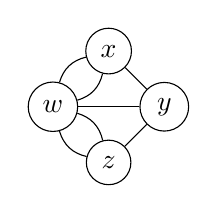
\begin{tikzpicture}[main/.style = {draw, circle}]
			\node[main] (w) {$w$};
			\node[main] (x) [above right of =w]{$x$};
			\node[main] (z) [below right of = w]{$z$};
			\node[main] (y) [above right of =z]{$y$};

			\draw (w) [bend right] to (x);
			\draw (x) [bend right] to (w);
			\draw (x) to (y);
			\draw (w) to (y);
			\draw (z) to (y);
			\draw (w) [bend right] to (z);
			\draw (z) [bend right] to (w);
		\end{tikzpicture}
		\caption{\label{fig:konigsberggraf} Graf til Königsberg Broer}
	\end{minipage}
\end{figure}

Vi vil nu definere hvad en \textit{graf} egentlig er.

\index{graf!definition}
\begin{definition}[Graf]
	En \textbf{graf} $G$ er en triple indeholdende knudemængden $V(G)$, en mængde af kanter $E(G)$ og en relation som associerer hver kant til to knuder, kaldet endepunkter.
\end{definition}

Jeg har allerede brugt ordene ``knuder'' og ``kanter''. I Figur~\ref{fig:konigsberggraf} kan man se et eksempel på en graf, hvor knuderne er repræsenteret af cirkler med et ``navn'' (inde i cirklen) og en kant der går mellem. Dette er den mest normale måde at repræsentere en graf på. Mængden af kanter er $\{w,x,y,z\}$ og mængden af kanter er unavngivet. En anden måde at definere en graf på er ved at bruge en 2-tuple (også kaldet et par), hvor knuderne forbliver defineret på samme måde, men kanterne i stedet defineres som en mængde af par, hvor parrene er to knuder. Her ville vi kunne definere kanterne som den følgende mængde: $\{(w,x), (x,w), (w,z), (z,w), (w,y), (x,y), (z,y)\}$. West bruger også denne notation, dog uden at gøre det til par, i.e. bliver vores mængde til $\{wx, xw, wz, zw, wy, xy, zy\}$

\index{graf!simpel}
\begin{definition}[Simpel Graf]
	En graf er \textbf{simpel} hvis måden kanterne sammensættes på kan ses som et par af uordnet knuder.
\end{definition}

Definitionen fra \href{https://www.georgmohr.dk/noter/grafteori2014.pdf}{Kristen Rosenkildes noter på grafteori} lægger også vægt i at der højest er en kant mellem to knuder (hvilket også kommer fra vores sammenligning) og at en knude ikke må gå til sig selv (løkke).

\index{graf!løkke}
\index{graf!multiple kanter}
\index{graf!nabokanter}
\begin{definition}[Løkke]
	En løkke er en kant hvis endepunkter er ens. Hvis et par af knuder har det samme par af endepunkter, kaldes de \textit{multiple kanter}. Når to kanter $u$ og $v$ er endepunkter af en kant er de \textit{naboer}\footnote{På engelsk siger man også at de to knuder er \textit{adjacent}.}. Vi skriver $u \leftrightarrow v$ til at mene ``$u$ og $v$ er nabokanter''.
\end{definition}

En graf er \textit{endelig} hvis mængden af kanter og knuder er endelige. Grafer i disse noter er endelige, undtagen hvis andet er sagt.

\index{graf!tom}
\begin{remark}
	\textit{Den tomme graf} (engelsk: null graph) er grafen hvis mængder af kanter og knuder er tomme. Den bliver generelt ikke brugt, og skal derfor ikke haves i baghovedet når man læser teksten.
\end{remark}

\subsection{Grafer som Modeller}%
\label{subsec:grafersommodeller}

Vi kan bruge grafer til at modellere mange problemer. Før vi går videre til et eksempel, giver vi definitionen på komplementet af en graf:
\index{graf!komplement}
\begin{definition}[Komplement af en graf]
	Komplementet $\overline{G}$ af en simpel graf $G$ er denne simple graf med knudemængden $V(G)$ defineret ved at $(u,v) \in E(\overline{G})$ hvis og kun hvis $(u,v) \in E(G)$.
\end{definition}

Vi kan nu se på et eksempel. Vi kan bruge grafer til at modellere om folk kender hinanden eller ej (ligeledes om deres forhold generelt: venner, fjender, bekendte, etc).


\begin{example}
	\label{ex:1.1.7}
	Har alle mængder af seks personer 3 fælles bekendte eller 3 fælles fremmede? Vi kan modellere dette med grafer, ved den viden at bekendtskaber er fælles. Hver knude repræsenterer en person, og hver kant et bekendtskab. Dermed, hvis der er en kant mellem to knuder er disse personer bekendte.
	\begin{figure}[H]
		\centering
		\begin{minipage}{0.45\textwidth}
			\centering
			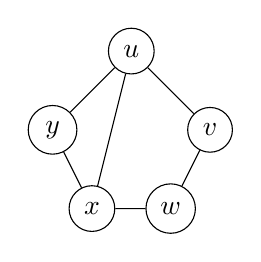
\begin{tikzpicture}[main/.style = {draw, circle}]
				\node[main] (u) at (0,0) {$u$};
				\node[main] (y) at (-1,-1) {$y$};
				\node[main] (x) at (-0.5,-2) {$x$};
				\node[main] (w) at (0.5,-2) {$w$};
				\node[main] (v) at (1,-1) {$v$};

				\draw (y) to (u)
				(u) to (v)
				(v) to (w)
				(w) to (x)
				(x) to (y)
				(u) to (x);

			\end{tikzpicture}
			\caption{\label{} Grafen $G$}
		\end{minipage}
		\hfill
		\begin{minipage}{0.45\textwidth}
			\centering
			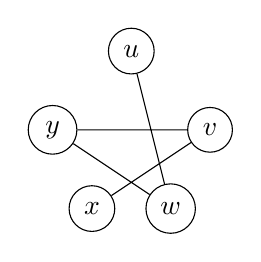
\begin{tikzpicture}[main/.style = {draw, circle}]
				\node[main] (u) at (0,0) {$u$};
				\node[main] (y) at (-1,-1) {$y$};
				\node[main] (x) at (-0.5,-2) {$x$};
				\node[main] (w) at (0.5,-2) {$w$};
				\node[main] (v) at (1,-1) {$v$};

				\draw (u) to (w)
				(w) to (y)
				(y) to (v)
				(v) to (x);

			\end{tikzpicture}
			\caption{Grafen $\overline{G}$}
		\end{minipage}
	\end{figure}
	Her kan vi se at komplementet, giver de personer der er fremmede endnu.
\end{example}



\index{graf!klikke}
\index{graf!uafhængig mængde}
\begin{definition}[Klikke, uafhængig mængde]
	En \textit{klikke} i en graf er en mængde af parvise naboknuder. En \textit{uafhængig mængde} (eller en stabil mængde) i en graf er en mængde af parvise knuder der \textbf{ikke} er naboer.
\end{definition}

Husk at to knuder er naboer når der er en kant imellem dem. Dermed kan du omformulere begge definition til at være følgende: En klikke er en delgraf hvor alle knuderne har kanter til alle andre knuder. En uafhængig graf er en delgraf hvor ingen af knuderne har kanter til nogen af de andre knuder.

I eksempel~\ref{ex:1.1.7} er $\{u,x,y\}$ en klikke af størrelse 3, og $\{u,w\}$ er en uafhængig mængde af størrelse 2. Under komplementet er disse omvendte, så $\{u,x,y\}$ er en uafhængig mængde, og $\{u,w\}$ er en klikke.

\index{graf!todelt}
\begin{definition}[Todelt Graf]
	En graf $G$ er todelt (bipartite) hvis $V(G)$ er foreningsmængden af to disjunkte uafhængige mængder kaldet \textit{delte mængder} (partite sets) af $G$.
\end{definition}

\begin{example}
	Hvis vi har $m$ jobs og $n$ personer, men ikke alle personer er kvalificeret til alle jobs, kan vi udfylde jobsne med kvalificeret personer? Vi kan modellere dette med en todelt graf, hvor jobs er en delgraf og personer er en anden. En person $p$ er nabo med job $j$ hvis $p$ er kvalificeret til $j$.
	\begin{center}
		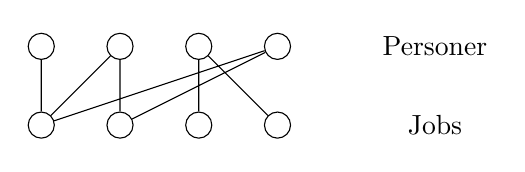
\begin{tikzpicture}[main/.style = {draw, circle}]
			\node[main] (p1) at (0,1) {};
			\node[main] (p2) at (1,1) {};
			\node[main] (p3) at (2,1) {};
			\node[main] (p4) at (3,1) {};
			\node (personer) at (5,1) {Personer};
			\node[main] (j1) at (0,0) {};
			\node[main] (j2) at (1,0) {};
			\node[main] (j3) at (2,0) {};
			\node[main] (j4) at (3,0) {};
			\node (jobs) at (5,0) {Jobs};

			\draw (p1) to (j1)
			(p2) to (j1)
			(p2) to (j2)
			(p3) to (j3)
			(p3) to (j4)
			(p4) to (j1)
			(p4) to (j2);
		\end{tikzpicture}
	\end{center}
\end{example}

\index{graf!kromatisk tal}
\begin{definition}[Kromatisk Tal]
	Det kromatiske tal af en graf $G$, skrevet $\chi(G)$ er minimumsantallet af farver nødvendige at give til knuder, således at naboknuder har forskellige farver.
\end{definition}

\index{graf!$k$-delelighed}
\begin{definition}[$k$-delelighed]
	En graf $G$ er $k$-delelig hvis $V(G)$ kan udtrykkes som foreningsmængden af (muligvis tomme) uafhængige mængder.
\end{definition}

\begin{example}
	Hvis vi har en mængde af komitéer, hvor nogle personer er i mere end en komité, og vi gerne vil planlægge tidspunktet for møder i disse komitéer, hvor mange forskellige tidspunkter skal vi bruge? Her er tidspunkterne farverne, så det minimum antal farver vi skal bruge, er også det minimum antal tidspunkter.
\end{example}

Vi kan bruge kromatiske tal til at generalisere todelelige grafer til $k$-delelige grafer. En graf er $k$-delelige hvis og kun hvis dens kromatiske tal er højest $k$. En delelig mængde (partite set på engelsk).

\index{graf!sti}
\begin{definition}[Sti]
	En \textit{sti} (path) er en simpel graf hvis knuder kan ordnes således at to knuder er naboer hvis og kun hvis de kommer efter hinanden i listen.
\end{definition}

Altså er en sti simpelt bare en graf hvor du kan gå fra knude $a$ til $b$ til $c$ etc.

\index{graf!kreds}
\begin{definition}[Kreds]
	En \textit{kreds} (cycle) er en graf med et lige antal af knuder og kanter, og hvor kanternes knuder kan blive placeret rundt i en cirkel således at to knuder er naboer hvis og kun hvis de er optræder efter hinanden i cirklen.
\end{definition}

\begin{example}
	Følgende er to grafer. Figur~\ref{fig:sti} er en sti, og Figur~\ref{fig:kreds} er en kreds.

	\begin{figure}[H]
		\centering
		\begin{minipage}{0.45\textwidth}
			\centering
			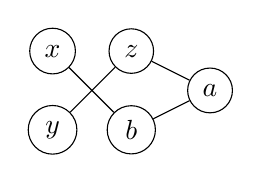
\begin{tikzpicture}[main/.style = {draw, circle}]
				\node[main] (x) at (0,0) {$x$};
				\node[main] (z) at (1,0) {$z$};
				\node[main] (a) at (2, -0.5) {$a$};
				\node[main] (y) at (0,-1) {$y$};
				\node[main] (b) at (1,-1) {$b$};

				\draw (x) to (b)
				(b) to (a)
				(a) to (z)
				(z) to (y);
			\end{tikzpicture}
			\caption{\label{fig:sti} En Sti}
		\end{minipage}
		\hfill
		\begin{minipage}{0.45\textwidth}
			\centering
			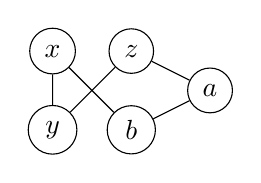
\begin{tikzpicture}[main/.style = {draw, circle}]
				\node[main] (x) at (0,0) {$x$};
				\node[main] (z) at (1,0) {$z$};
				\node[main] (a) at (2, -0.5) {$a$};
				\node[main] (y) at (0,-1) {$y$};
				\node[main] (b) at (1,-1) {$b$};

				\draw (x) to (b)
				(b) to (a)
				(a) to (z)
				(z) to (y)
				(y) to (x);
			\end{tikzpicture}
			\caption{\label{fig:kreds} En Kreds}
		\end{minipage}
	\end{figure}
	Bemærk her, at hvis man fjerner én kant fra en kreds bliver det til en sti.
\end{example}

Når vi snakker om stier og kredse er det ofte i forbindelse med om der er en sti eller kreds i en graf som i sig selv ikke er en sti eller en kreds.

\index{graf!delgraf}
\begin{definition}[Delgraf]
	En \textit{delgraf} af en graf $G$ er en graf $H$ hvor $V(H) \subseteq V(G)$ og $E(H) \subseteq E(G)$, og at tildelingen af endepunkter til kanter i $H$ er det samme som i $G$. Vi siger ``G \textit{indeholder} H'' og skriver $H \subseteq G$.
\end{definition}

\index{graf!sammenhængende}
\begin{definition}[Sammenhængende Graf]
	En graf $G$ er sammenhængende hvis hvert par af knuder i $G$ hører til en sti, ellers er $G$ usammenhængende.
\end{definition}

En måde at tænke på en sammenhængende graf på, er ved at spørge om man kan opdele de to eller flere grafer i hver deres mængder af knuder, uden at miste nogle kanter. Hvis dette \textit{ikke} er muligt, er grafen sammenhængende. Ellers er den usammenhængende.


\subsection{Matricer og Isomorfi}%
\label{subsec:label}

Vi har set hvordan vi kan specificere grafer ved at tegne cirkler som knuder og streger som kanter, men der er andre måder at gøre det på. En graf er \textit{løkkeløs} hvis multiple kanter er tilladt, men løkker ikke er. I Figur~\ref{fig:pp7g} kan grafen ses, som vil bruges til at vise hvordan man ellers kan repræsentere en graf.


\index{graf!repræsentationer!nabo-matrix}
\begin{definition}[Nabo-matrix]
	Lad $G$ være en løkkeløs graf med knudemængden $V(G) = \{v_{1}, \ldots, v_{n}\}$ og kantemængden $E(G) = \{e_{1}, \ldots, e_{m}\}$. Nabo-matricen af $G$, skrevet $A(G)$ er en $n \times n$ matrix hvori hver post i matricen $a_{i,j}$ er antallet af knuder i $G$ med endepunkterne $\{v_{i}, v_{j}\}$.
\end{definition}

\begin{figure}[H]
	\vspace{-20pt} % Adjusts the vertical space
	\centering
	\begin{tikzpicture}
		\graph [spring layout, nodes={circle, draw}] {
		w --[edge label={$a$}] x,
		w --[edge label={$b$}] y,
		x --[bend left, edge label={$d$}] y,
		y --[bend left, edge label={$c$}] x,
		y --[edge label={$e$}] z
		};
	\end{tikzpicture}
	\caption{\label{fig:pp7g} $G$}
\end{figure}


Følgende er nabo-matricen for grafen $G$ i Figur~\ref{fig:pp7g}:
\begin{equation}
	A(G) = \begin{pmatrix}
		0 & 1 & 1 & 0 \\
		1 & 0 & 2 & 0 \\
		1 & 2 & 0 & 1 \\
		0 & 0 & 1 & 0
	\end{pmatrix}
\end{equation}

\index{graf!repræsentationer!incidens-matrix}
\begin{definition}[Incidens-matrix]
	Incidens-matricen af $G$, skrevet $M(G)$  er en $N \times m$ matrix hvori post $m_{i,j}$ er 1 hvis $v_{i}$ er et endepunkt af $e_{j}$, og ellers 0.
\end{definition}

Bemærk at en nabo-matrix er \textit{symetrisk} altså, $a_{i,j} = a_{j,i}$ for alle $i,j$, det vil sige at der ikke kan være rettet kanter\footnote{Vi har endnu ikke snakket om rettet grafer, kun urettet.}.

Følgende er incidens-matricen for $G$ i Figur~\ref{fig:pp7g}:
\begin{equation}
	M(G) = \begin{pmatrix}
		1 & 1 & 0 & 0 & 0 \\
		1 & 0 & 1 & 1 & 0 \\
		0 & 1 & 1 & 1 & 1 \\
		0 & 0 & 0 & 0 & 1
	\end{pmatrix}
\end{equation}

\index{graf!incidens}
\index{graf!valens}
\begin{definition}[Incidens og Valens]
	Hvis knude $v$ er et endepunkt af kant $e$, så er $v$ og $e$ \textit{incidente}. Valensen (også kaldet graden, \textit{degree} på engelsk) af knuden $v$ af antallet af incidente kanter, minus løkker.
\end{definition}

\index{graf!isomorfi}
\begin{definition}[Isomorfi]
	En \textit{isomorfi} fra en simpel graf $G$ til en simpel graf $H$ er en bijektion $f : V(G) \rightarrow V(H)$ hvor $(u,v) \in E(G)$ hvis og kun hvis $(f(u), f(v)) \in E(H)$. Vi siger at ``$G$ er isomorfisk til $H$'', skrevet $G \cong H$, hvis der er en isomorfi fra $G$ til $H$.
\end{definition}

\begin{example}[Isomorfi fra $G$ til $H$]
	Vi kigger nu på et eksempel, på hvordan en graf $G$ kan blive isomorfisk til en graf $H$.

	\begin{center}
		\begin{tikzpicture}
			\graph [spring layout, nodes={circle, draw, minimum size=0.8cm}] {
				w[x=0,y=0] -- x[x=0,y=-2],
				x -- y[x=2,y=0],
				y -- z[x=2,y=-2]
			};
		\end{tikzpicture}
	\end{center}

	Vi definerer nu en funktion som tager alle knuderne i $G$ og laver dem om til knuderne i en graf $H$: $f : V(G) \rightarrow V(H)$, $f(w) = a, f(x) = d, f(y) = b, f(z) = c$.
	Dette giver grafen:
	\begin{center}
		\begin{tikzpicture}
			\graph [spring layout, nodes={circle, draw, minimum size=0.8cm}] {
				c[x=0,y=0] -- b[x=2,y=-2],
				b -- d[x=2,y=0],
				d -- a[x=0,y=-2]
			};
		\end{tikzpicture}
	\end{center}
	Bemærk her, at trods knuderne i en anden ``rækkefølge'' end tidligere, er det en isomorfi. Vi kan verificere dette ved at lave en nabo-matrix til begge, og se hvordan vi kan ændre nabo-matricen til at gøre det mere klart.\footnote{Desværre gør \LaTeX\ det ikke nemt at lave etiketter til matricer, så i stedet skriver vi det som en tabel.}
	\begin{equation}
		A(G) =
		\begin{array}{c|cccc}
			  & w & x & y & z \\
			\hline
			w & 0 & 1 & 0 & 0 \\
			x & 1 & 0 & 1 & 0 \\
			y & 0 & 1 & 0 & 1 \\
			z & 0 & 0 & 1 & 0 \\
		\end{array}
	\end{equation}
	\begin{equation}
		A(H) =
		\begin{array}{c|cccc}
			  & a & b & c & d \\
			\hline
			a & 0 & 0 & 0 & 1 \\
			b & 0 & 0 & 1 & 1 \\
			c & 0 & 1 & 0 & 0 \\
			d & 1 & 1 & 0 & 0 \\
		\end{array}
	\end{equation}
	Bemærk dog at de ikke er helt ens. Vi kan gøre dem ens, ved at omarrangere etiketterne:
	\begin{equation}
		A(G) =
		\begin{array}{c|cccc}
			  & w & y & z & x \\
			\hline
			w & 0 & 0 & 0 & 1 \\
			y & 0 & 0 & 1 & 1 \\
			z & 0 & 1 & 0 & 0 \\
			x & 1 & 1 & 0 & 0 \\
		\end{array}
	\end{equation}
\end{example}

Ud fra dette eksempel kan vi se, at to grafer, $A(H)$ og $A(G)$ er isomorfiske hvis og kun hvis deres nabo-matricer har en permutation af rækker og kolonner \(\sigma\), hvor $A(H)$ og $A(G)$ er ens.

Vi har indtil nu kun identificeret isomorfi for simple grafer, men det er også muligt for grafer med multiple kanter og løkker at være isomorfiske:

\begin{definition}[Isomorfi for ikke-simple grafer]
	En isomorfi fra $G$ til $H$ er en bijektion $f$ som afbilder $V(G)$ til $V(H)$ og $E(G)$ til $E(H)$ således at hver kant af $G$ med endepunkter $u$ og $v$ er afbildet til en kant med endepunkter $f(u)$ og $f(v)$.
\end{definition}

Bemærk \textit{at være isomorfisk} er ikke muligt i sig selv. En graf $G$ kan ikke være isomorfisk, men et par af grafer, $G$ og $H$ kan være isomorfiske til hinanden.

\index{mængde!relation}
\index{mængde!ækvivalensrelation}
\begin{definition}
	En \textit{relation} på en mængde $S$ er en samling af orndet par fra $S$. En \textit{ækvivalensrelation} er en relation som er refleksiv, symmetrisk og transitiv.
\end{definition}

For eksempel er nabo-relationen på en mængde af knuder af en graf symmetrisk, men ikke releksiv og sjældent transitiv. Dog er den isomorfiske relation, indeholende mængden af ordnet par ($G, H$) hvor $G$ er isomorfisk til $H$ både transitiv, symmetrisk og refleksiv.

\begin{proposition}
	Den isomorfiske relation er en ækvivalensrelation på mængden af simple grafer.
\end{proposition}

\begin{proof}
	\textit{Refleksiv}: Identitetspermutationen på $V(G)$ er en isomorfi fra $G$ til selg selv, dermed $G \cong G$.\footnote{Jeg forstår ikke helt det her. Identitetspermutation betyder bare at hver mængde afbilder til sig selv i en mængde.} \\
	\noindent
	\textit{Symmetrisk}: Hvis $f : V(G) \rightarrow V(H)$ er en isomorfi fra $G$ til $H$ så er $f^{-1}$ en isomorfi fra $H$ til $G$, fordi udsagnet ``$(u,v) \in E(G) \iff (f(u),f(v)) \in E(H)$'' giver $(x,y) \in E(H)$ hvis og kun hvis $f^{-1}(x)f^{-1}(y) \in E(H)$. Dermed $G \cong H \implies H \cong G$\\
	\noindent
	\textit{Transitiv}: Antag at $f : V(F) \rightarrow V(G)$ og $g : V(G) \rightarrow V(H)$ er isomorfier. Vi er givet udsagnet ``$(u,v) \in E(F) \iff (f(u), f(v)) \in E(G)$'' og ``$(x,y) \in E(G) \iff (g(x),g(y)) \in E(H)$''. Siden $f$ er en isomorfi, for hvert $(x,y) \in E(G)$ kan vi finde $(u,v) \in E(F)$ således at $f(u) = x$ og $f(v) = y$. Dette giver ``$uv \in E(F) \iff (g(f(u)),g(f(v))) \in E(H)$''.
\end{proof}



\index{graf!isomorfi!isomorfisme klasse}
\begin{definition}
	En \textit{isomorfisme klasse} af grafer er en ækvivalensklasse af grafer under isomorfismerelationen.
\end{definition}


\index{graf!komplet}
\index{graf!$n$-kreds}
\index{graf!todelelig!komplet}
\begin{definition}[Komplet graf, $n$-kreds]
	Stien og kredesen med $n$ knuder skrives henholdsvis $P_{n}$ og $C_{n}$. En $n$-kreds er en kreds med $n$ knuder. En \textit{komplet graf} er en graf hvis knuder er parvise naboer, og skrives $K_{n}$ for $n$ knuder. En \textit{komplet todelelige graf}, også kaldet \textit{biklikke} (biclique på engelsk) er en todelelig graf hvor to knuder er naboer hvis og kun hvis de er i forskellige delelige mængder. Når mængderne har størrelser $r$ og $s$ skrives biklikken $K_{r,s}$.
\end{definition}

Den komplette graf kan også forklares som værende grafen hvor alle knuder har kanter til alle andre knuder.

Figurene~\ref{fig:k23pp9} og~\ref{fig:k5pp9} viser henholdsvis en biklikke, $K_{2,3}$, og en komplet graf, $K_{5}$. Bemærk at jeg har navngivet knuderne, trods dette ikke er nødvendigt i disse eksempler. Bogen bemærker endda i definitionen at dette gælder umærket grafer.


\begin{figure}[H]
	\centering
	\begin{tikzpicture}
		\graph [spring layout, nodes={circle, draw, minimum size=0.8cm}] {
			a[x=0,y=0] -- c[x=-1,y=-2],
			c -- b[x=2,y=0],
			b -- d[x=1, y=-2],
			b -- e[x=3, y=-2],
			e -- a -- d
		};
	\end{tikzpicture}
	\caption{\label{fig:k23pp9} $K_{2,3}$}
\end{figure}

\begin{figure}[H]
	\centering
	\begin{tikzpicture}
		\graph [spring layout, nodes={circle, draw, minimum size=0.8cm}] {
		a -- {b, c, d, e},
		b -- {c, d, e},
		c -- {d, e},
		d -- {e}
		};
	\end{tikzpicture}
	\caption{\label{fig:k5pp9} $K_{5}$}
\end{figure}

I en graf med en mængde af knuder $X$ som har størrelse $n$, kan hvert par af knuder blive til en kant, eller det kan ikke. Antallet af grafer med mængden af knuder $X$ er $2^{\binom{n}{2}}$, fordi der er $2^{\binom{n}{2}}$ forskellige måder at vælger kanter mellem knuderne på. Hvis, for eksempel, $n = 4$, så er der $2^{\binom{4}{2}} = 2^{6} = 64$ forskellige grafer med den mængde af knuder.

\subsection{Nedbrydning og Specielle Grafer}%
\label{subsec:label}

\index{graf!selv-komplementær}
\index{graf!nedbrydning}
\begin{definition}[Selv-komplementær og Nedbrydning]
	En graf er \textit{selv-komplementær} hvis den er isomorfisk til dens komplement. En \textit{nebdrydning} af en graf er en liste af delgrafer hvor hver kant opstår i præcis en delgraf i listen.
\end{definition}

Denne definition kan nemt misforstås. Jeg foretrækker at tænke på det som ``En nebdrydning af en graf er en liste af delgrafer, hvor kanterne forbliver de samme par, og ingen af knuderne fjernes, således at foreningsmængden af disse delgrafer giver den originale graf.''
Ud fra denne definition, er det klart at en $n$-knude graf $H$ er selv-komplementær hvis og kun hvis den komplette graf med $n$ knuder, $K_{n}$ har en nedbrydning af to kopier af $H$.

\begin{definition}[Petersen Grafen]
	Petersen grafen er grafen hvis knuder er delmængder af 2 elementer af en mængde med 5 elementer, og hvis kanter er par af disjunkte delmængder af 2 elementer.
\end{definition}

Definitionen er lidt indviklet, så jeg vil komme med et eksempel. Givet en mængde med 5 elementer, $S = \{1, 2, 3, 4, 5\}$, er der $\binom{5}{2} = 10$ forskellige knuder. En af måderne vi kan gøre dette på giver os knuderne $V = \{12, 34, 51, 23, 45, 13, 35, 52, 24, 41\}$. Der er $\binom{3}{2}$ disjunkte delelementer af størrelse 2, så hver knude har 3 naboer. Vi definerer naboerne til at være de par som er disjunkte 2-element delmængder. Dermed, hvis vi har knuden $12$, vil de resterende elementer, i.e. naboerne, være $34, 45, 35$. Dette gør vi ved alle knuder. Antallet af kanter i alt er så $|E| = \frac{1}{2} \sum \text{deg}(v) = \frac{1}{2} (3 \cdot 10)  = 15$.

\begin{figure}[ht]
	\centering
	\begin{tikzpicture}[every node/.style={draw,circle, minimum size=0.8cm}]
		\graph[clockwise, radius=2cm] {subgraph C_n [n=5,name=A]};
		\graph[clockwise, radius=1cm] {subgraph I_n [n=5,name=B]};

		\foreach \i in {1,2,3,4,5}{\draw (A \i) -- (B \i);}
		\newcounter{j}
		\foreach \i in {1,2,3,4,5}{%
				\pgfmathsetcounter{j}{ifthenelse(mod(\i+2,5),mod(\i+2,5),5)}
				\draw (B \i) -- (B \thej);
			}
	\end{tikzpicture}
	\caption{\label{fig:petersengraf} Petersen Graf}
\end{figure}

I Figur~\ref{fig:petersengraf} ses en Petersengraf, dog med tvetydige etikketer.

\begin{proposition}
	\label{prop:petersenonecommon}
	Hvis to knuder ikke er naboer i Petersengrafen, så har de præcis én nabo.
\end{proposition}

\begin{proof}
	Knuder som ikke er naboer er mængder af størrelse 2, som deler ét element. Deres fællesmængde $S$ har størrelse 3. Dette er fordi naboerne er de eneste knuder som ikke deler elementer. Siden de mængder af størrelse 2 er valgt fra $\{1,2,3,4,5\}$, er der præcis én mængde af størrelse 2 som er disjunkt fra $S$.
\end{proof}

\index{graf!omkreds}
\begin{definition}[Omkreds]
	\textit{Omkredsen} (engelsk: girth) af en kraf med en kreds er længden af dens korteste kreds. En graf uden kreds er uendelig omkreds.
\end{definition}

\begin{corollary}
	Petersengrafen har omkreds 5.
\end{corollary}
\begin{proof}
	Da grafen er simpel (uden løkker eller multiple kanter) har den ingen 1-kreds eller 2-kreds. En 3-kreds ville kræve tre parvise disjunkte mængder af størrelse 2, hvilket ikke er muligt med 5 elementer, som i Petersengrafen.
	En 4-kreds kræver ikke-nabo-knuder med to ens naboer, hvilket Proposition~\ref{prop:petersenonecommon} viser værende umuligt.
	Knuderne $12, 34, 51, 23, 45$ giver en 5-kreds, så omkredsen er 5.
\end{proof}

Petersengrafen er meget symmetrisk. Hver permutation af $\{1,2,3,4,5\}$ genererer en permutation af delmængder af størrelse 2, som opretholder disjunktrelationen. Dermed er der mindst $5! = 120$ isomorfismer fra Petersengrafen til sig selv.

\index{graf!automorfisme}
\index{graf!knudetransitiv}
\begin{definition}[Automorfi og Knudetransitiv]
	En \textit{automorfi} af $G$ er en isomorfi fra $G$ til $G$. En graf $G$ er \textit{knudetransitiv}, hvis, for hvert par $(u,v) \in V(G)$ er der en automorfi som afbilder $u$ til $v$.
\end{definition}

%%% Local Variables:
%%% mode: latex
%%% TeX-engine: luatex
%%% TeX-command-extra-options: "-shell-escape"
%%% TeX-master: "main"
%%% End:
